\documentclass{article}
\usepackage[english,russian]{babel}
\usepackage[utf8]{inputenc}
\usepackage{indentfirst}
\usepackage{graphicx}
\usepackage{float}
\usepackage[margin=2cm]{geometry}

\begin{document}
\begin{titlepage}
	\begin{center}
    	ГУАП
    	\vspace{0.25cm}

    	КАФЕДРА №51
	\end{center}

    \begin{flushleft}

    	ОТЧЕТ

    	ЗАЩИЩЕН С ОЦЕНКОЙ

		ПРЕПОДАВАТЕЛЬ


    	\vspace{0.5cm}

		$\rule{5cm}{0.15mm}$ \hfill $\rule{2.2cm}{0.15mm}$  \hfill $\rule{3.25cm}{0.15mm}$

		должность, уч. степень, звание \hfill подпись, дата \hfill инициалы, фамилия
    \end{flushleft}

 	
    \hspace{2cm}

	\begin{center}
    	ОТЧЕТ ПО ЛАБОРАТОРНОЙ РАБОТЕ №9


    	\vspace{1cm}

    	SYNCHRONIZED


    	\vspace{1cm}

    	по курсу: ОСНОВЫ ПРОГРАММИРОВАНИЯ {\MakeUppercase{\romannumeral 2}}
    \end{center}

    \vspace{3cm}

    \begin{flushleft}
    	РАБОТУ ВЫПОЛНИЛ

    	СТУДЕНТ ГР. № 5511 \hfill $\rule{2.2cm}{0.15mm}$  \hfill $\rule{3.25cm}{0.15mm}$

    	\hspace{7.8cm} подпись, дата \hfill инициалы, фамилия
    \end{flushleft}

	\vspace{5cm}
	\begin{center}
 		Санкт-Петербург, 2017
	\end{center}
\end{titlepage}

\section{Задание}
Написать программу, приводящую к ситуации взаимной блокировки (deadlock).


\section{Дополнительное задание}
Реализовать программу которая подсчитывает статистику употребления слов в заданных текстовых файлах. Программа получает список файлов в качестве параметров командой строки. Каждый файл обрабатывается в отдельном потоке. Для подсчета числа уникальных слов используется общий для всех потоков HashMap.

\section{Реализация}
Для получения ситуации deadlock'a были созданы классы Account и AccountTransfer. Эти классы позволяли симулировать какую-то часть банковских операций, а именно снятие и добавление средств с счёта и на счёт. \\

Класс AccountTransfer наследовался от класса Thread, в конструкторе потока указывались аккаунты для совершения транзакции и сумма транзакции. В методе run() синхронизировались сначала один аккаунт, а затем второй (внутри блока synchronized первого аккаунта). Но при запуске нескольких потоков с использованием одних и тех же аккаунтов возникала ситуация взаимной блокировки, так как для того, чтобы отпустить 1 замок необходимо, чтобы 2 замок был опущен, но он не может быть опущен, так как не опущен 1 замок. И так получилось, что два потока ждут пока один из них освободит один из замков и программа не работает как должна. \\

В дополнительной программе, которая подсчитывает статистику употребления слов были созданы новые классы CalculateFileStat, WordFinder и WordStat. \\

CalucalteFileStat принимает имена файлов для сканирования в аргументах программы, а затем запускает потоки WordFinder'a отнаследованного от класса Thread. WordFinder хранит в себе статистику WordStat (одну на все потоки), которая предается ему в конструкторе. Для предотвращения ошибок доступа к ресурсу необходимо было использовать блок synchronized. 


\section{Инструкция}
При запуске основной программы последовательно выводит на экран:\\
Getting info from Alice's account\\
Getting info from Eva's account\\
Дальше происходит блокирование программы.

При запуске дополнительной программы выводит на экран HashMap хранящий в качестве ключа слово и в качестве значения частоту этого слова в текстах.

\section{Тестирование}

\subsection{Пример запуска основной программы}
\begin{figure}[H]
	\begin{flushleft}
		\centerline{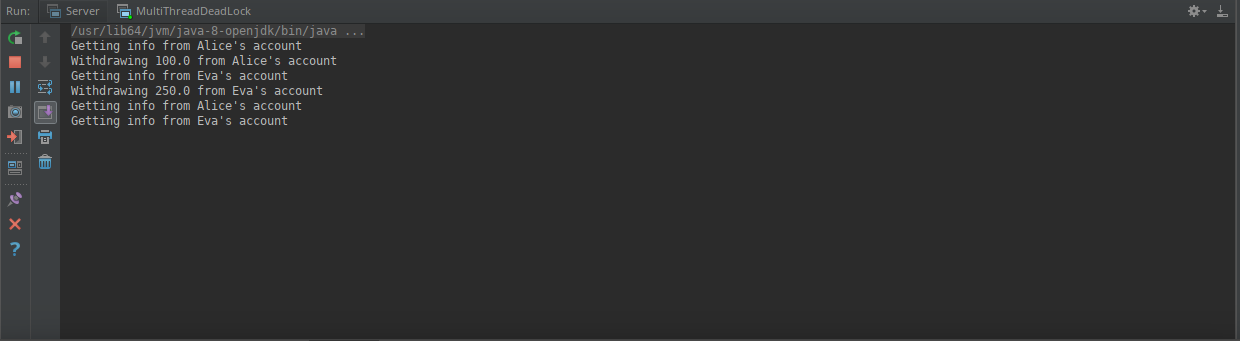
\includegraphics[scale=0.55]{lab9_main.png}}
		\caption{Пример запуска основной программы}
	\end{flushleft}
\end{figure}
\vspace{3cm}

\subsection{Пример запуска дополнительной программы}
\begin{figure}[H]
	\begin{flushleft}
		\centerline{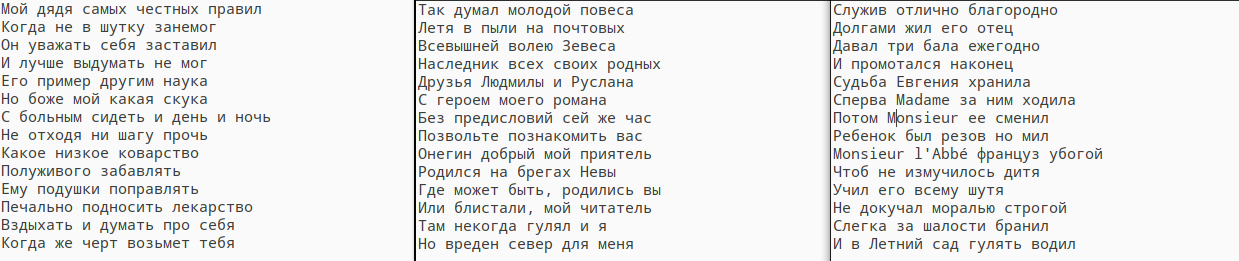
\includegraphics[scale=0.55]{example.png}}
		\caption{Пример входных текстов}
        \vspace{3cm}
        \centerline{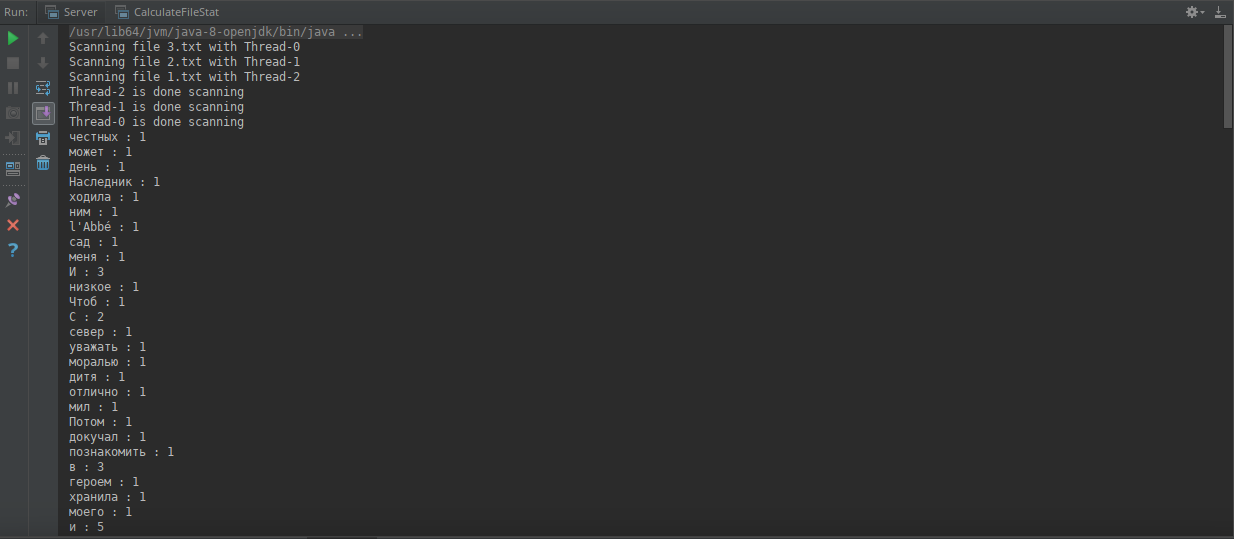
\includegraphics[scale=0.55]{lab9_add.png}}
		\caption{Пример запуска дополнительной программы}
	\end{flushleft}
\end{figure}


\end{document}
